\section{AliEn}

AliEn \cite{AliEn} is a set of middleware tools and services which represents
an implementation of the ALICE distributed computing environment
integrated in the WLCG environment. AliEn has been under a constant
development by ALICE since 2001 and was deployed over the
ALICE Grid infrastructure right from the start. One of the important
features is the set of interfaces to other Grid implementations like
gLite \cite{glite}, ARC \cite{arc} and OSG \cite{OSG}.

AliEn was initially developed as a distributed production
environment for the simulation, reconstruction, and analysis of
Physics data. Since it was put in the production in 2001, ALICE has
been using AliEn before the start of  the real data taking for
distributed production cycles of Monte-Carlo simulated raw data,
including subsequent reconstruction and analysis, during the regular
Physics Data Challenges. Since 2005, AliEn has been used also for
end-user analysis.  Since December 2007, when the ALICE detector
started operation taking cosmic data, AliEn has been used also for
management of the raw data.  Since the LHC startup in 2009, millions
of jobs have been successfully processed using the AliEn services
and tools.

AliEn developers provided the users with a client/interface - ``alien
shell'' \cite{alienshell} and a set of plugins designed for the end users' job
submission and handling. These tools together with the tools
provided by the ALICE Grid monitoring framework MonALISA \cite{MonALISA}, hide
the complexity and heterogenity of the underlying Grid services from
the end-user while facing the rapid development of the Grid
technologies.

AliEn is a lightweight Open Source Grid framework built around Open
Source components using the combination of standard network
protocols, a Web Service and Distributed Agent Model. The basic
AliEn components include:
%
\begin{itemize}
\item AliEn File Catalogue with metadata capabilities
\item  Data management tools for data transfers and storage
\item Authentication, authorization and auditing services
\item Job execution model
\item Storage and computing elements
\item Information services
\item Site services
\item Command line interface - the AliEn shell aliensh
\item ROOT interface
\item Grid and job monitoring
\item Interfaces to other Grids
\end{itemize}

AliEn was primarily developed by ALICE, however it was adopted also
by a couple of other Virtual Organizations like PANDA \cite{PANDA} and CBM \cite{CBM}.

\subsection{File Catalogue (FC)}
%
The File Catalogue is one of the key components of the AliEn suite.
It provides a hierarchical structure (like a UNIX File system) and
is designed to allow each directory node in the hierarchy to be
supported by different database engines, running on different hosts.
This building on top of several databases allows to add another
database to expand the catalogue namespace and assures scalability
of the system and allow growth of the catalogue as the files
accumulate over the years.

Unlike real file systems, the FC does not own the files; it is a
metadata catalogue on the Logical File Names (LFN) and only keeps an
association/mapping between the LFNs and (possibly multiple)
Physical File Names (PFN) of real files on a storage system. PFNs
describe the physical location of the files and include the access
protocol (rfio, xrootd), the name of the AliEn Storage Element and
the path to the local file. The system supports file replication and
caching.

The FC provides also a mapping between the LFNs and Globally Unique
Identifiers (GUID). The labeling of each file with the GUID allows
for the asynchronous caching. The write-once strategy combined with
GUID labeling guarantees the identity of files with the same GUID
label in different caches. It is possible to automatically construct
PFNs : to store only the GUID and Storage Index and the Storage
Element builds the PFN from the GUID. There are two independent
catalogues: LFN->GUID and GUID->PFN. A schema of the AliEn FC is
shown in Figure~\ref{fig15}.

%fig15
\begin{figure}[htb] % h-here, t-top, b-bottom
\centering
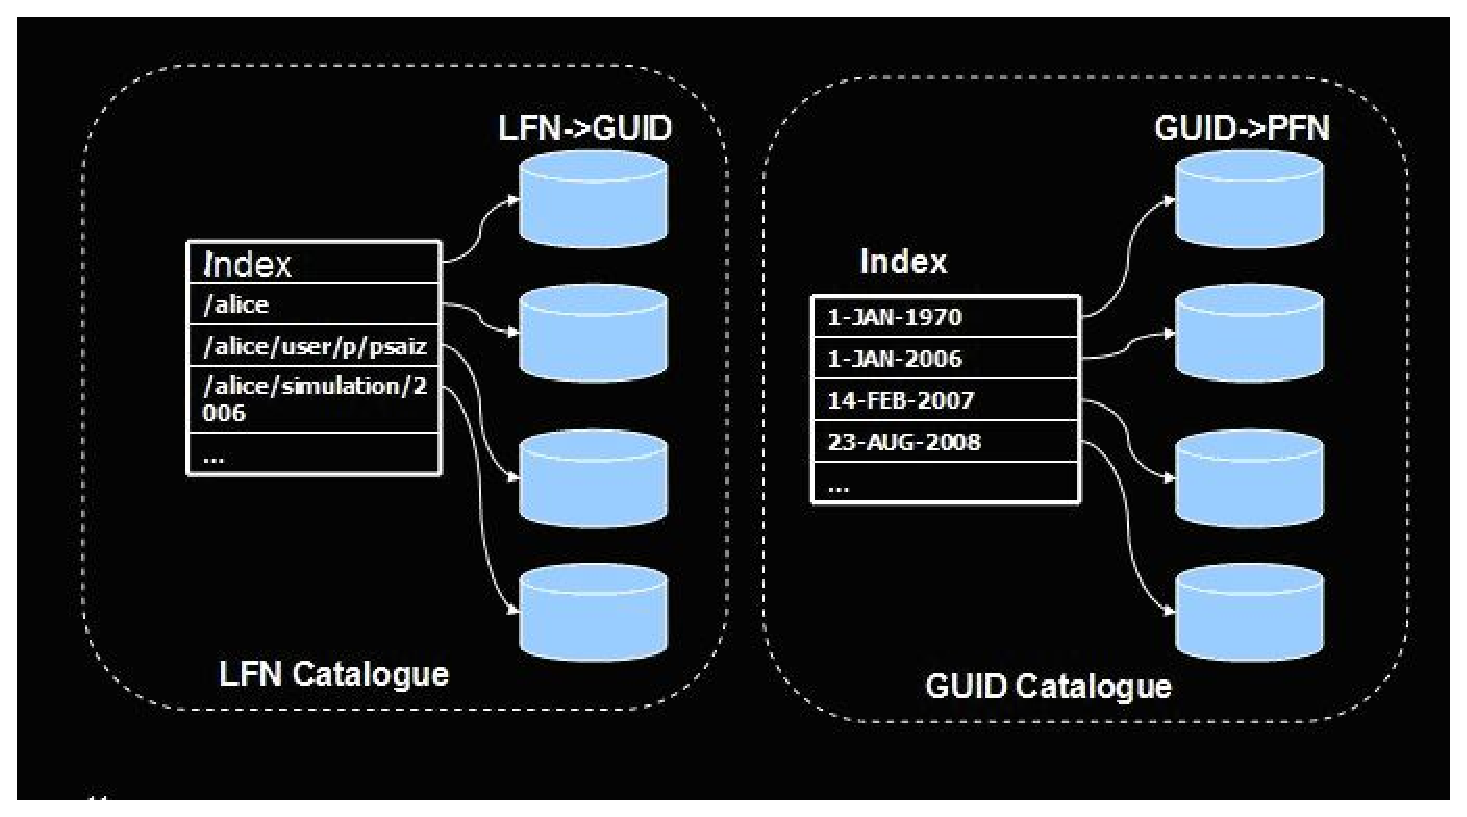
\includegraphics[width=13cm]{fig15.eps} %    ** if .eps don't need extension
\caption{AliEn File Catalogue}\label{fig15}
\end{figure}

The FC can also associate metadata to the LFNs. This metadata is a collection of
user-defined key value pairs. For instance, in the case of ALICE, the current metadata is 
the software version used to generate the files, number of events inside a file, or 
calibration files used during the reconstruction.


\subsection{Job execution model}
%
AliEn's Job execution model is based on the pull
architecture. There  is a set of central components (Task Queue, Job
Optimizer, Job Broker) and another set of  site components (Computing Element (CE),
Cluster Monitor, MonALISA, Package Manager). The pull architecture
has one major advantage with respect to the push one: the system does not have to
know the actual status of all resources, which is crucial for large
flexible Grids. In a push architecture, the distribution of jobs requires to 
keep and analyze a huge amount of status data just to assign a job,
which becomes difficult in the expanding grid environment. In the
pull architecture, local agents (pilot status-checking test jobs)
running at individual sites ask for real jobs after having checked
the local conditions and found them
appropriate for the processing of the job. Thus, AliEn only deals
with the requests of local pilot jobs, so called Job Agents (JA), to
assign appropriate real jobs. The descriptions of jobs in the form
of ClassAds are managed by the central Task Queue.

Each site runs several AliEn services: CE, ClusterMonitor,
Package Manager (PackMan) and a MonALISA client. The AliEn CE
automatically generates Job Agents and submits them to the local batch system. 

The ClusterMonitor manages the connections between
the site and central services, so there is only one connection from
each site. The AliEn CE can also be submit to the CREAM-CE, ARC, OSG  or even the WMS, 
and delegate the communication with the local batch system to such a service.
 Schemas of the job submission procedure in
AliEn are shown in Figures~\ref{fig16} and~\ref{fig17}.

%fig16
\begin{figure}[htb] % h-here, t-top, b-bottom
\centering
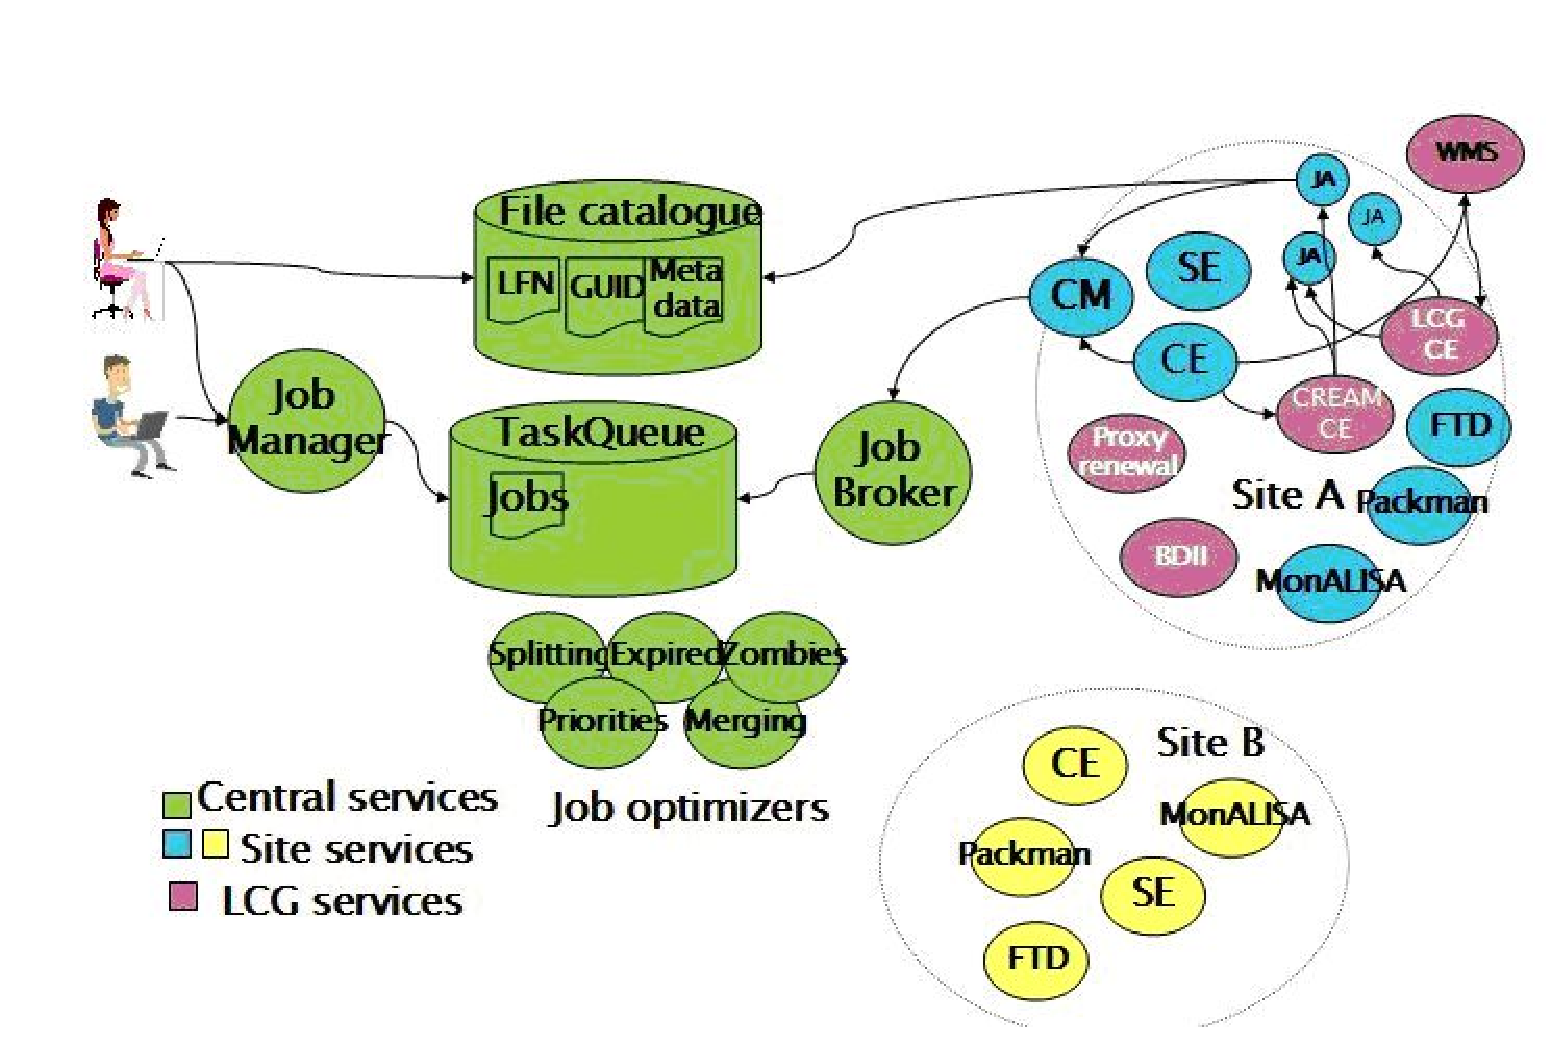
\includegraphics[width=13cm]{fig16.eps} %    ** if .eps don't need extension
\caption{AliEn + WLCG services}\label{fig16}
\end{figure}



%fig17
\begin{figure}[htb] % h-here, t-top, b-bottom
\centering
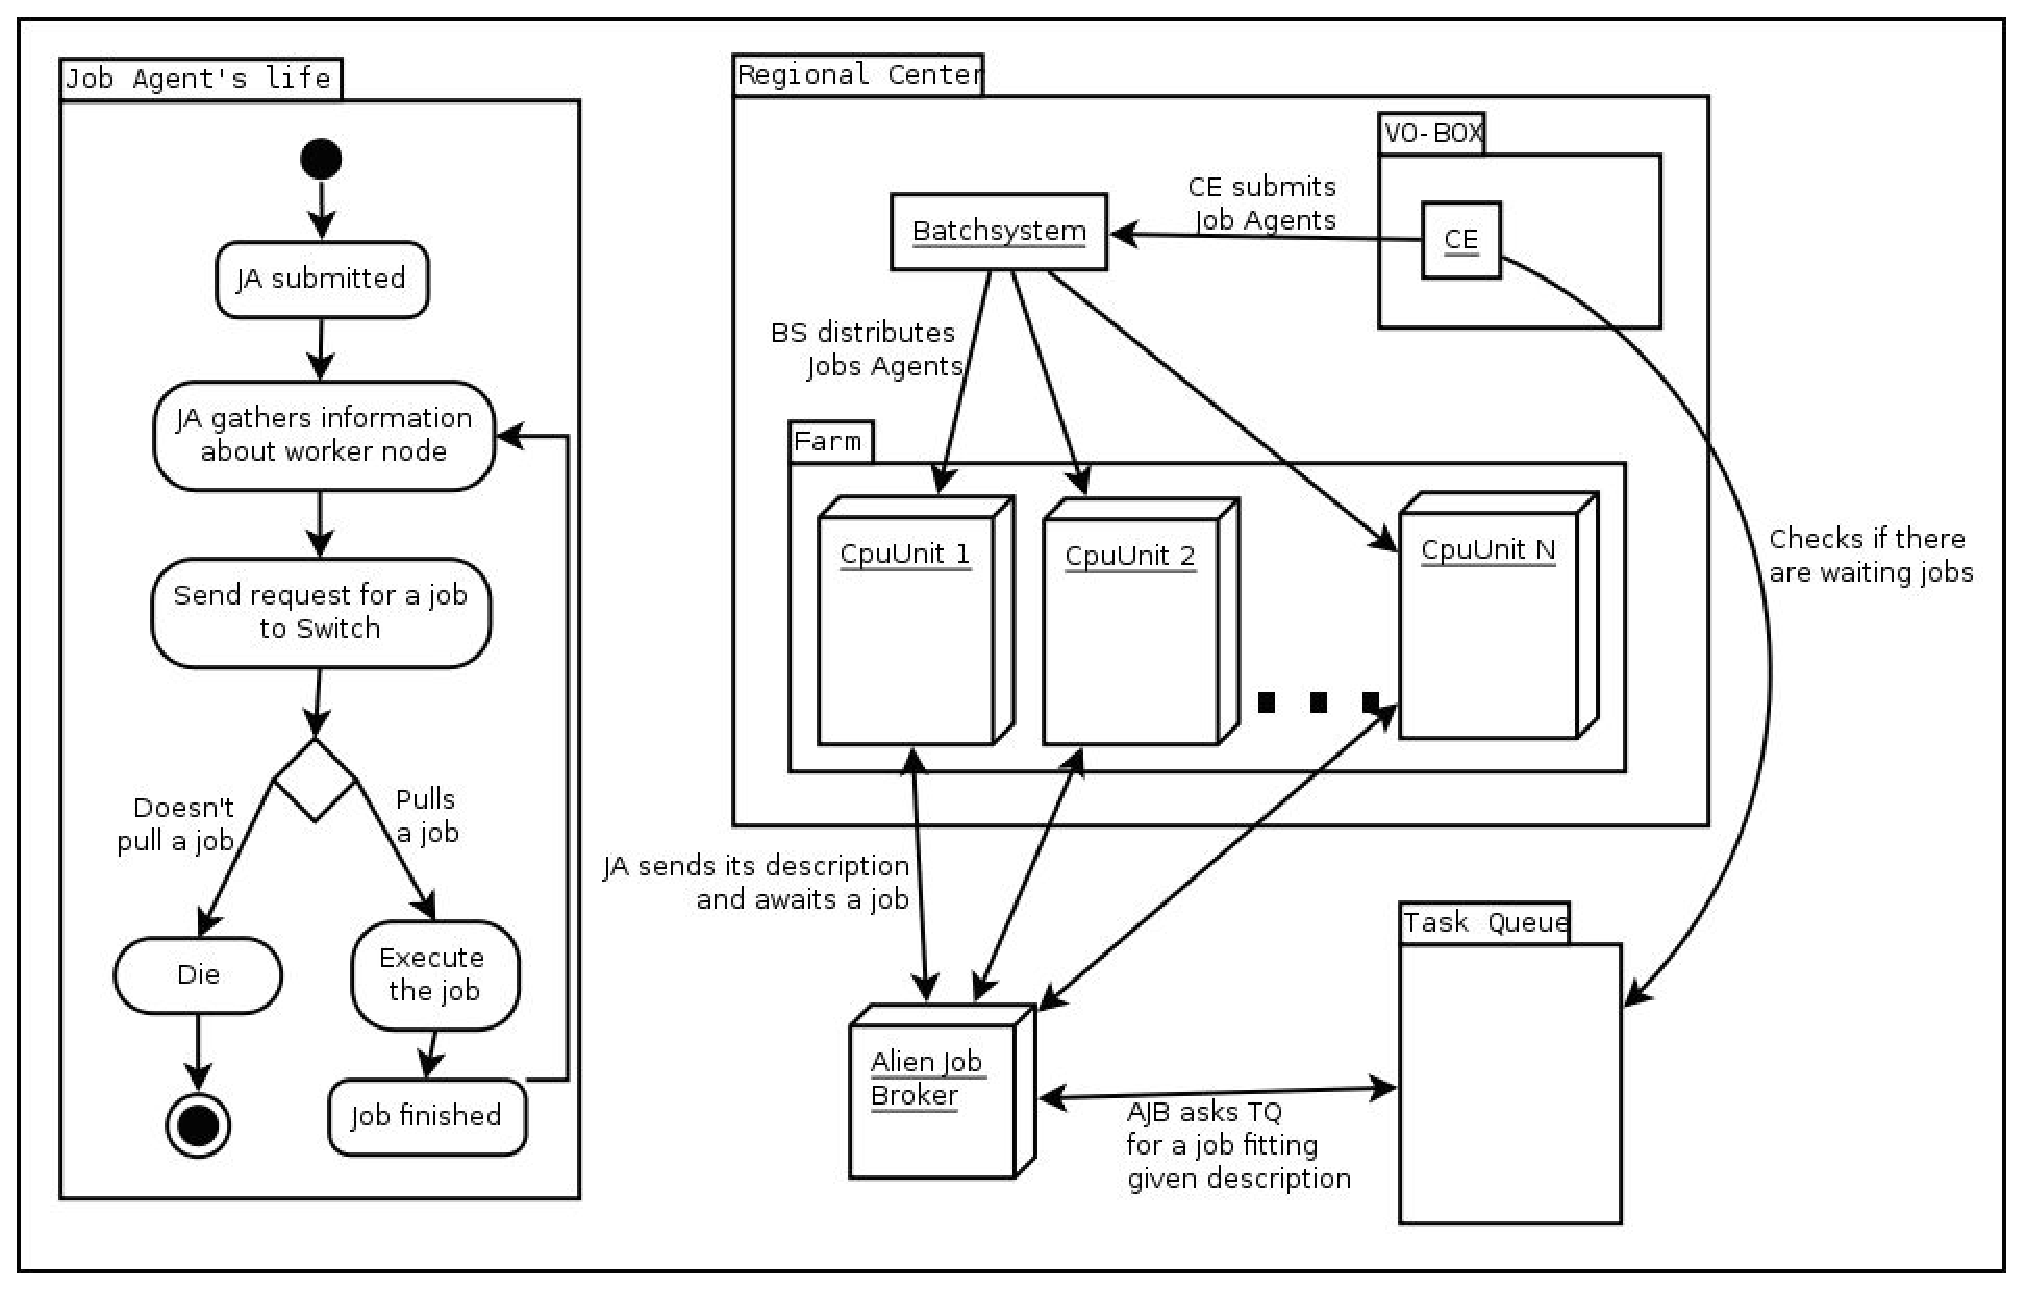
\includegraphics[width=13cm]{fig17.eps} %    ** if .eps don't need extension
\caption{The Job Agent model in AliEn}\label{fig17}
\end{figure}



\subsection{Jobs}
%
When a job is submitted by a user, its description in the form of a
ClassAd is kept in the central TQ  where it waits for a suitable Job Agent for execution.  
There are several Job optimizers that can rearrange the priorities of the jobs based 
on the user quotas. These optimizers can also split jobs,  or even 
suggest data transfers so it would be more likely that some Job
Agent picks up the job.

After it has been submitted, a job gets through several stages \cite{job_status}.  The information about running processes is kept also in the
AliEn FC. Each job is given a unique id and a corresponding
directory where it can register its output. The JAs provide a job-wrapper, a standard environment
allowing a virtualization of resources. The whole job submission and
processing chain is extensively monitored so a user can any time get
the information on the status of his/her jobs.

\subsection{Site services}
%
As mentioned before, there are several AliEn services running at each ALICE site: 
CE, ClusterMonitor, PackMan and MonALISA.
These services are running on a dedicated machine, so called VOBOX
described in section 3.

The AliEn site CE is usually associated with the local batch system.
It is periodically submitting testing pilot jobs (Job Agents)  to
the local WLCG CE or an appropriate external Resource Broker or WMS.
The role of the Job Agents is to verify the local hardware and
software capacities at the site. After the usual matchmaking
procedure, the JA is sent, through the site CE, into the local batch
queue and then to a local Worker Node (WN). After its startup, the
JA performs its task and in the case of a positive checkup, the JA
requests a "real" job from the central Task Queue via the AliEn Job
Broker, or dies otherwise.

The PackMan automates the process of installation, upgrades,
configuration and removal of the ALICE software packages from the
shared software area on the site. It also advertises known/installed
packages. The packages are installed on demand, when requested by a
Job Agent running on a Worker Node or during the central software
deployment over the Grid sites. If a package is not already
installed the PackMan would install it along with its dependencies
and return a string with commands that client has to execute to
configure the package and all its dependencies. The PackMan manages
the local disk cache and cleans it, when it needs more space to
install newer packages.

The Cluster Monitor handles communication with the AliEn Job Broker
and gives configuration to JAs.  It gets ``heartbeats'' from the JAs.
If it gets no heartbeats from a JA, the existing job will get into
the ZOMBIE status (after 1.5 hours) and then it will expire (after 3 hours).

\subsection{Monitoring}
%
Since the AliEn Workload Management does not
depend directly on sophisticated monitoring, no special monitoring
tools were developed in AliEn. As the monitoring solution, ALICE has
adopted and further developed the Java-based MonALISA framework
mentioned already in the previous section. The MonALISA system is
designed as an ensemble of autonomous multithreaded, self-describing
agent-based subsystems which are registered as dynamic services, and
together can collect and process large amounts of information.

The collected monitoring information is published via Web Service
for use by AliEn Optimizers or for visualization purposes. An
extension of the network simulation code which is a part of MonALISA
can provide a tool for optimization and understanding of the
performance of the AliEn Grid system.

\subsection{Storage}
%
Experience with the performance of different types of storage
managers shows that the most advanced storage solution is the native
XRootD manager described in section 3. It has been demonstrated
that with all other parameters being equal (protocol access speed
and security) the native XRootD storage clusters exhibit
substantially higher stability and availability. The ALICE
distributed system of native XRootD clusters is orchestrated by the
global redirector which allows interacting with the complete storage
pool as a unique storage.  All storages are on WAN (Wide Area
Network).

\subsection{AliEn Shell - aliensh}
%
To complete the brief description of AliEn, we mention the client
called AliEn shell. It provides a UNIX-shell-like environment with
an extensive set of commands which can be used to access AliEn Grid
computing resources and the AliEn virtual file system.  There are
three categories of commands: informative and convenience commands,
File Catalogue and Data Management commands and TaskQueue/Job
Management commands. The AliEn shell has been created about 4 years
ago and become a popular tool among the users for job handling and
monitoring.

\subsection{Concluding remarks}
%
AliEn is a high-level middleware adopted by
the ALICE experiment, which has been used and validated in massive
Monte Carlo events production since 2001, in end-user analysis since
2005 and during the real data management and processing since 2007.
Its capabilities comply with the requirements of the ALICE computing
model. In addition to modules needed to build a fully functional
Grid, AliEn provides interfaces to other Grid implementations
enabling the true Grid interoperability. The AliEn development will
be ongoing in the coming years following the architectural path
chosen at the start and more modules and functionalities are
envisaged to be delivered.

The Grid (AliEn/gLite/other) services are many and quite complex.
Nonetheless, they are working together, allowing to manage thousands
of CPUs and PBs of various storage types. The ALICE choice of single
Grid Catalogue, single Task Queue with internal prioritization and a
single storage access protocol (xrootd) has been beneficial from
user and Grid management viewpoint.

